\documentclass[10pt]{article}

% Packages
\usepackage{enumerate}
\usepackage{mathptmx}
\usepackage{helvet}
\usepackage{listings}
\usepackage[left=0.75in,right=0.75in,top=0.875in,bottom=0.875in]{geometry}
\usepackage{titling}
\usepackage{tabularx}
\usepackage{multicol}
\usepackage[explicit]{titlesec}
\usepackage{graphicx}
\usepackage{xcolor}

% Single column figure
\newenvironment{InlineColumnFigure}
{\par\medskip\noindent\minipage{\linewidth}}
{\endminipage\par\medskip}

% Caption
\newcommand{\Caption}[1]
{\vspace{-4mm}\fontsize{9}{9}\textbf{Figure \refstepcounter{figCounter} 
\arabic{figCounter}: #1}}

\newcounter{figCounter}
\setcounter{figCounter}{0}

% ACM CHI Format
\setlength{\columnsep}{0.85cm}
\setlength{\parindent}{0pt}

\titlespacing{\section}{0pt}{10pt}{-\parskip}
\titlespacing{\subsection}{0pt}{10pt}{-\parskip}
\titlespacing{\subsubsection}{0pt}{10pt}{-\parskip}

\titleformat{\section}{\normalfont\fontsize{9}{9}\sffamily\bfseries}
{\thesection}{1em}{\MakeUppercase{#1}}
\titleformat{\subsection}{\normalfont\fontsize{9}{9}\sffamily\bfseries}
{\thesubsection}{1em}{#1}
\titleformat{\subsubsection}{\normalfont\fontsize{9}{9}\sffamily\itshape}
{\thesubsubsection}{1em}{#1}

\pagenumbering{gobble}

%===============================- 80 columns -=================================%
\begin{document}

% Title
\begin{center}
{\LARGE \sffamily \textbf{Course-Management System: Final Report} 
\vspace{2mm}}\\
\begin{tabular}{cccc}
\textbf{Stuart Douglas} & \textbf{Matthew Pagnan} & \textbf{Rob Gorrie} & 
\textbf{Derek Dagworthy}\\
1214422 & 1208693 & 1222547 & 1214937\\
McMaster University & McMaster University & McMaster University & McMaster 
University\\
dougls2@mcmaster.ca & pagnanmm@mcmaster.ca & gorrierw@mcmaster.ca & 
dagwordj@mcmaster.ca\\
\end{tabular}
\end{center}
\vspace{2mm}

\begin{multicols}{2}

% =================== Section =================== -------------- Change This
\section*{Abstract}
A \emph{design} final report for a course-management system is presented 
here. Such a system allows University students to enroll in courses, view their 
schedule and perform other course-related tasks from a web portal. The proposed 
project as well as suggested improvements are first explained. Four Canadian 
university course-management software surveys are then presented. Each survey 
has a brief description followed by a critique of the major usability flaws and 
strengths. Three personas are then presented to give the reader an idea of the 
people likely to be using this system. A section for information about the usablily 
tests conducted for this system is presented next followed by a result, a discussion
and a conclusion section about the results obtained from the usability tests
% =================== Section =================== %
\section*{Project Proposal}

% =================== SubSection =================== % --------- Rob -- condense and change to past tense
The project proposed in this document is the design of a new 
university course-management system. Through scrutinization of several 
pre-existing systems, we will apply design concepts discussed in class to 
determine what features and design choices are crucial to the success of a course-
management system's design.

It is commonplace for educational institutions to have one central course-
management system which hosts all tools and information that students and staff 
may need to access. This includes tools to allow students to enroll in courses, 
view their schedule and view other course-related information. Additionally 
there are a variety of other tools to perform financial and administrative 
tasks, however this project's scope is focusing only on the course-related 
functions.

Course-management systems have achieved near omnipresence in 
the world of education, but there remains significant variability in their design, 
structure, and functionality. It is our goal to take the best aspects of the 
existing systems as well as consider the most prominent criticisms to develop a protoype of a new system.

In the following section we will introduce several possible improvements that 
could be made to these systems, informed by the system surveys below. It is 
these suggestions that we plan to incorporate into prototypes for later 
milestones.

% =================== SubSection =================== %
\subsection*{Suggested Improvements to Existing Systems}
There were a variety of improvements that have been made to the course-management 
system when compared to existing products. The software surveys identified 
several key areas of weaknesses, and solutions to those are presented below.

\subsubsection*{Dynamic Element}
One of the highlighted points of weakness in all the systems surveyed was the 
ability to surface the most relevant data to the user quickly and consistently. 
To improve this aspect, the concept of an intelligent, ``dynamic'' element was 
proposed. This prominent element is the first thing users see when 
accessing the webpage. Several factors including the current date and enrollment 
status were used to determine which task the user is most likely to perform.

For example, when the user accesses the system during exam season, the element 
 displays the student's exam schedule. During the course registration period, 
the element displays information related to course registration. If a user 
is not yet accepted into University, the element displays their application 
status.

This dynamic element helps users quickly find the information they are 
looking for by making information more visible and easier to access. All functions continue to be 
displayed below in a static and consistent manner, in case the user wishes to perform a less common task.

\subsubsection*{Improved Navigation}
Many tasks performed by users of course-management software are broken into 
several steps. A weakness of the existing products was in visually showing the 
user at which step they were at. A navigation element was included for when the user is engaged in a multi-step task.
This element shows which step the user is currently on, and includes the ability to 
go back to a previous step, or jump ahead to the first uncompleted step.

This visual indicator improves the user's comprehension of how the system 
works, and gives them the ability to better navigate between steps. It also improves user satisfaction, 
as they are less likely to become impatient when they know exactly 
how many steps they have completed and how many remain. 

% =================== Section =================== %
\section*{Software Survey}
Four course-management systems from Canadian universities were selected for 
review. For each system, a brief description was followed by a critique of 
the major usability flaws and strengths. From this, the main goals and tasks of 
users using the systems was extracted. 

%Finally, the two most important of 
%those features was further analyzed via hierarchical task analyses. 
%Screenshots were presented to reinforce the arguments in the critique for 
%each software review.

% =================== SubSection =================== %
\subsection*{McMaster University -- Mosaic}

\subsubsection*{Description}
The purpose of the software is to allow students to manage their courses 
(enrolling, dropping etc.), and view information about their current status 
(current timetable, enrollment status, financial balance etc.). The main 
interface for the software consists of several collapsible modules 
encapsulating different aspects of the software in a main column. These include 
Academics, Finances, Personal Information, and Admissions. A small column to 
the right holds less common sections, such as Enrollment Dates and Graduation. 
The focus of this analysis is on two common tasks -- enrolling in courses and 
viewing one's course schedule.

%\begin{InlineColumnFigure}
%\begin{center}
%	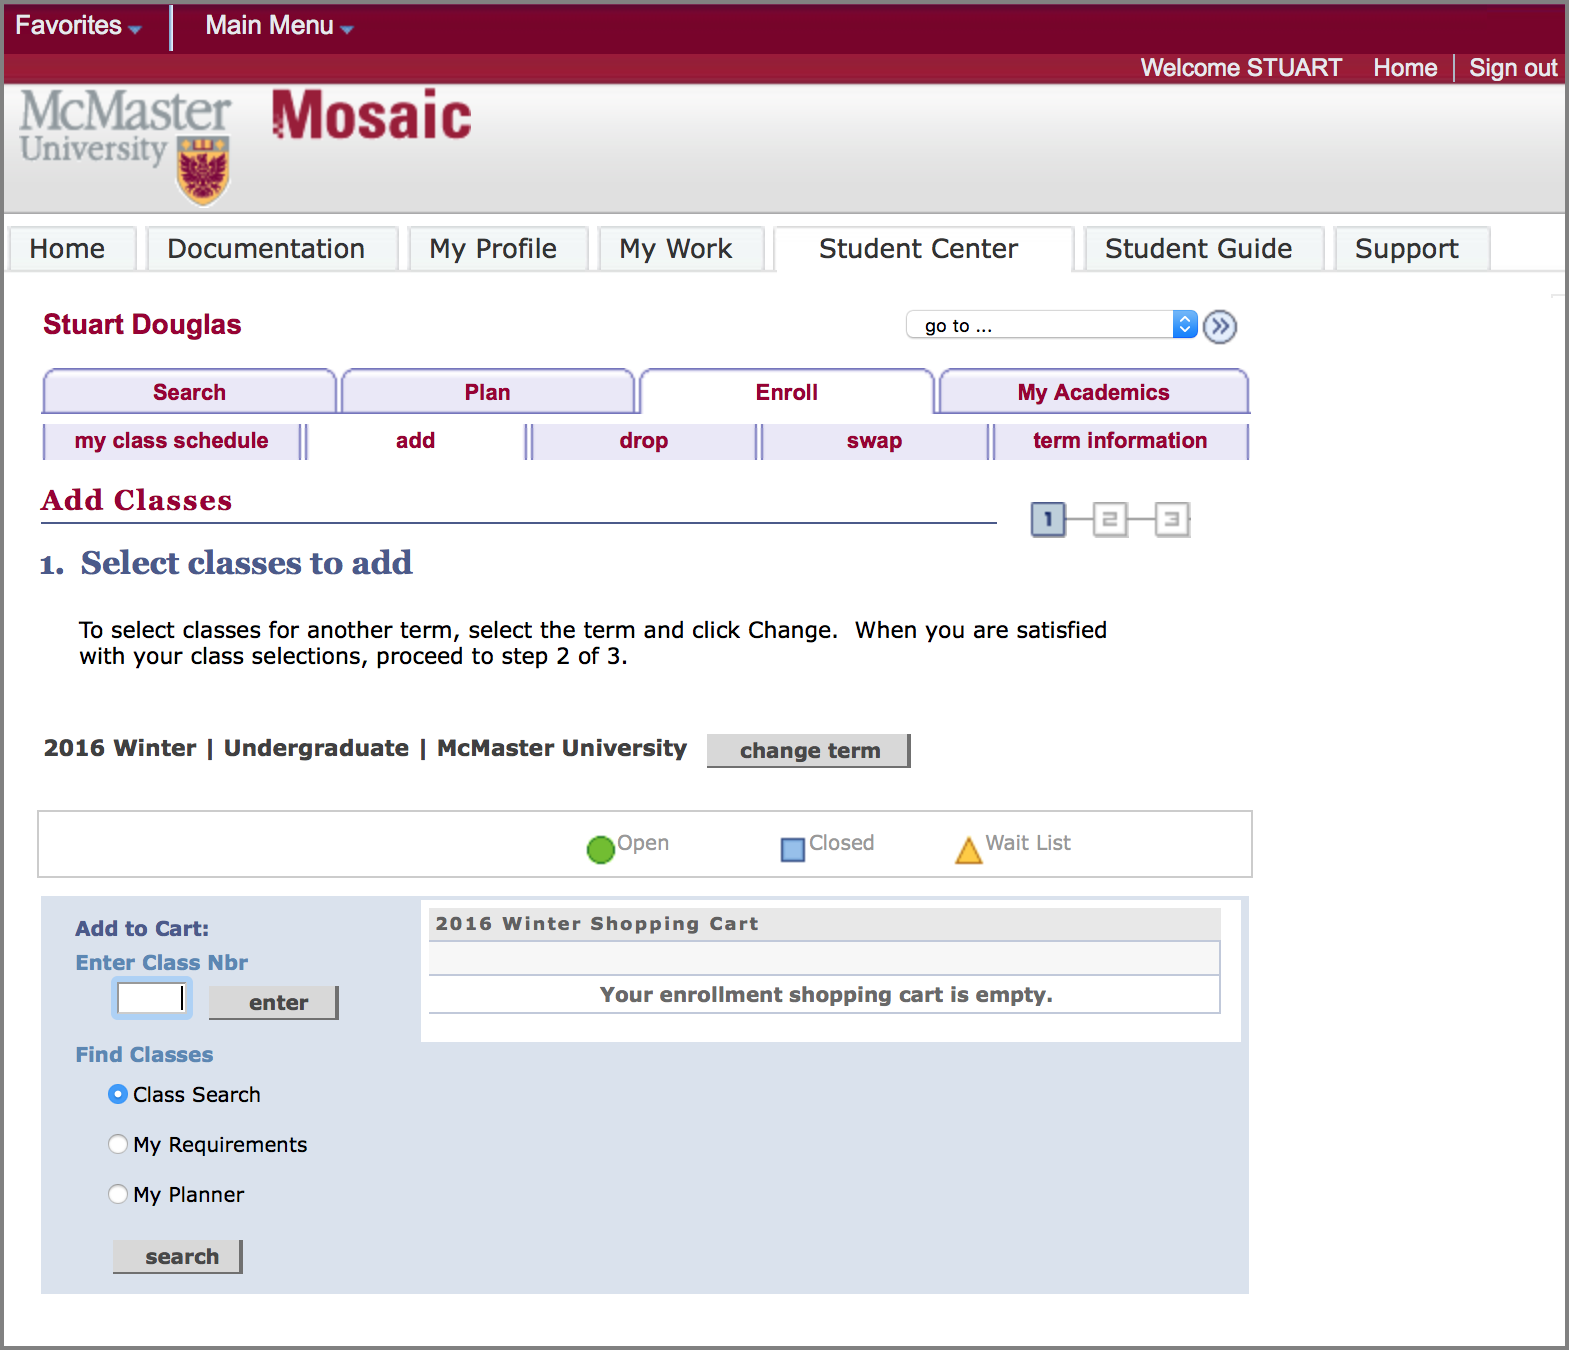
\includegraphics[width=0.8\textwidth]{MosaicScreen.png}
%\end{center}
%\Caption{Selecting courses to enroll in -- Mosaic}
%\end{InlineColumnFigure}

\subsubsection*{Critique}
The largest usability flaws in Mosaic center around difficulty to access 
required information. Combined with an unintuitive and inconsistent navigation 
interface, the software is . The HTA for enrolling in a course demonstrates this 
through the large number of steps required to perform a routine and common task. 
Other functions are hidden behind dropdown menus, and are difficult to discover.


The navigation is separated into a top navigation bar separated by user-type 
(e.g. Students and Employees). Within the student center page, functions are 
separated into modules, an effective strategy to group related functions. 
Navigating to one of the sub-functions (such as enrolling in a course) presents 
secondary and tertiary menus below the main one. Navigation within one of these 
is handled by blue text hyperlinks back to previous pages. Native back and 
forward browser functionality does not work. There is little visual indication 
of where the user is beyond the navigation bars at the top, which do not go to a 
depth sufficient to cover all pages used when performing common actions, such as 
enrolling in a course.

% =================== SubSection =================== %
\subsection*{Guelph University -- WebAdvisor}
\subsubsection*{Description}
Guelph University's course enrollment software, WebAdvisor, provides a variety 
of functions for students to manage their courses. The student page interface 
contains two columns -- a main column with course-related news, and a righthand 
column with links to each of the functions (Register for Courses, View Schedule 
etc). These ``function'' pages are one column, and may contain several sub-pages 
as processes are broken into steps. Navigating between sub-pages is done using 
native browser back and forward buttons. If an error occurs, such as no courses 
found for specific search criteria, a large box is displayed with information 
about the error and the option to search for a solution.

%\begin{InlineColumnFigure}
%\begin{center}
%	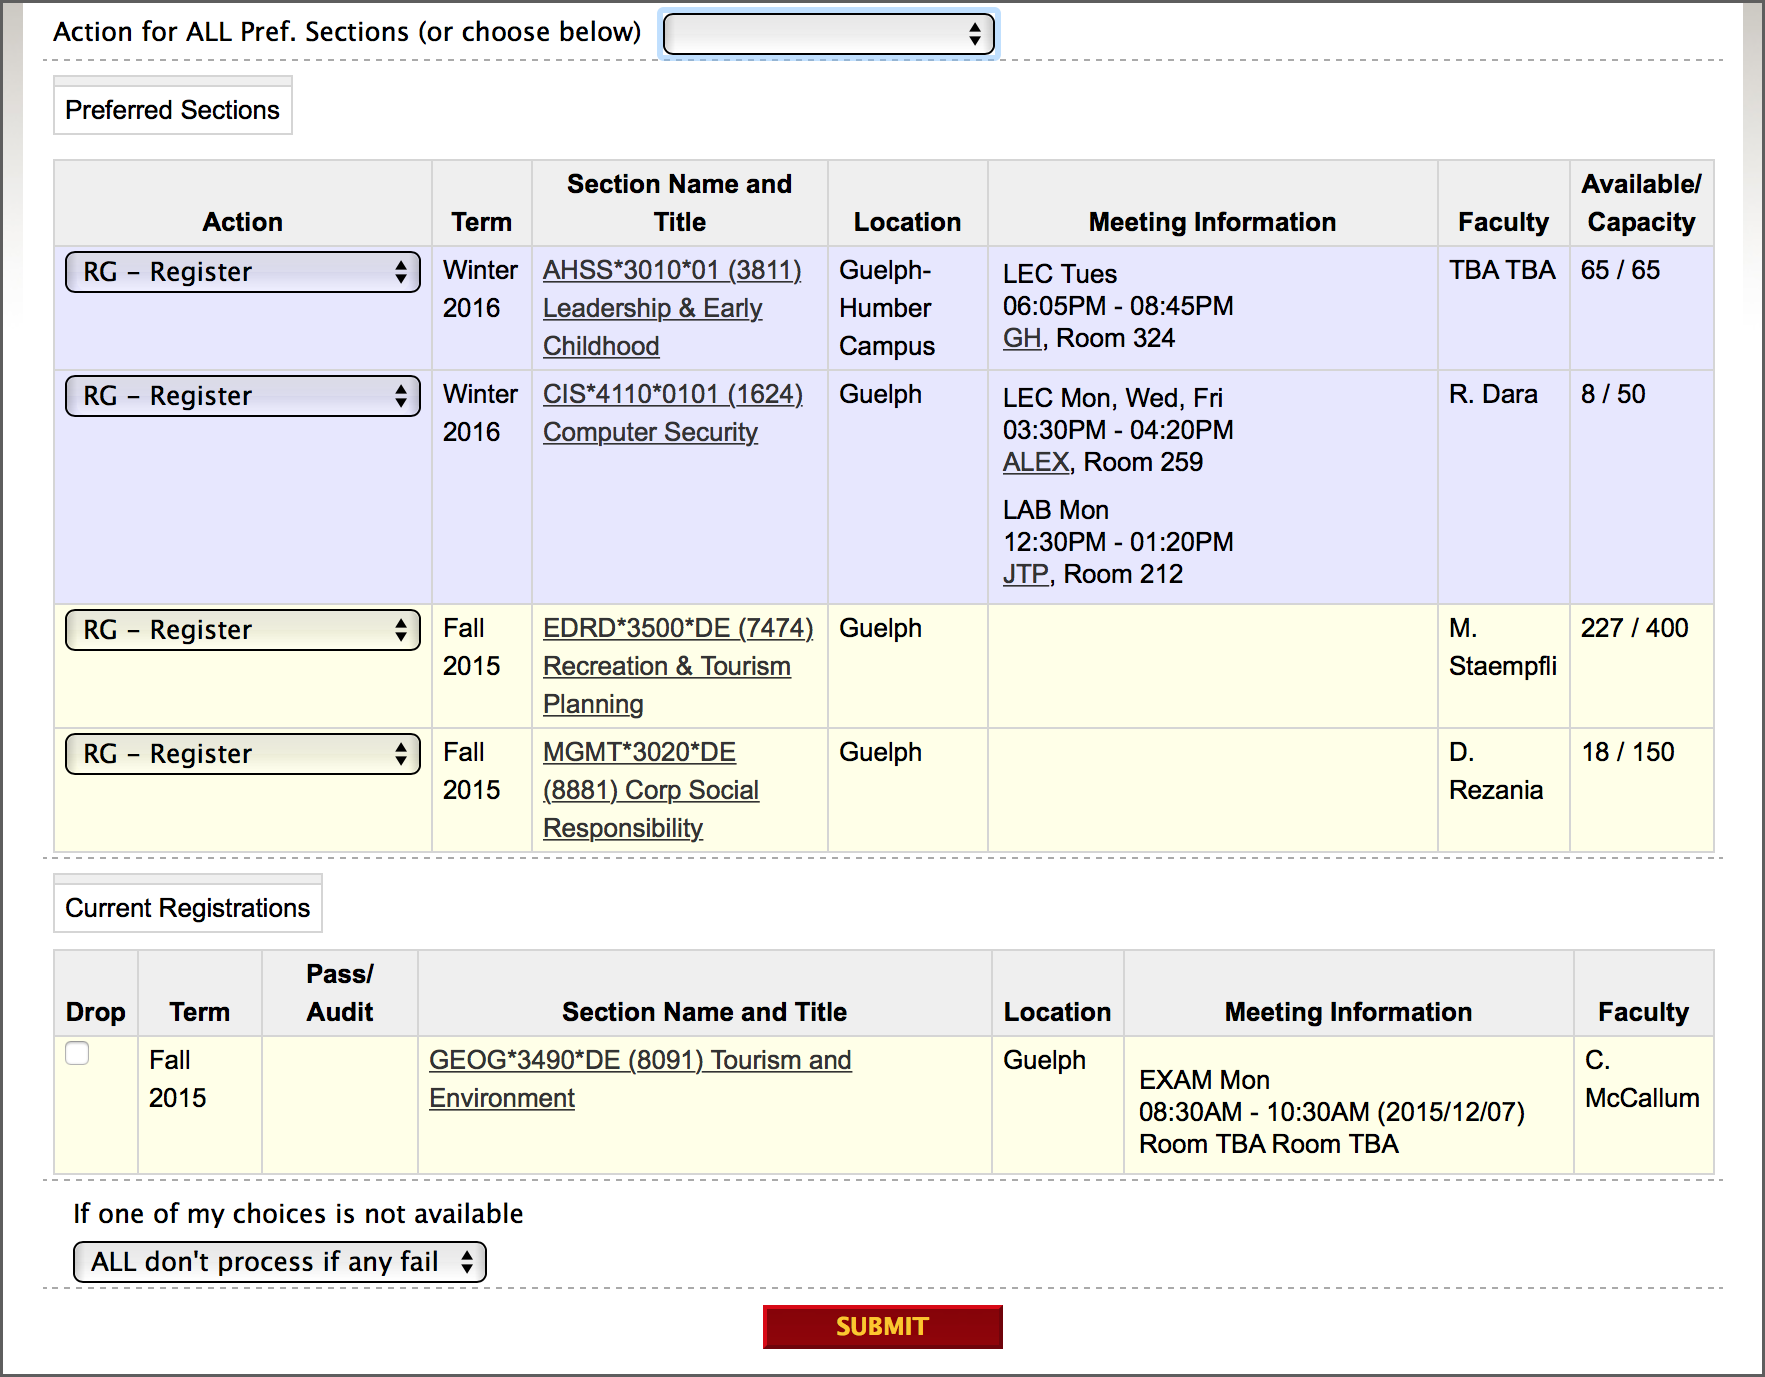
\includegraphics[width=0.9\textwidth]{WebAdvisorScreen.png}
%\end{center}
%\Caption{Registering for preferred courses -- WebAdvisor}
%\end{InlineColumnFigure}

\subsubsection*{Critique}
There are a variety of usability issues associated with \mbox{WebAdvisor} that 
could be improved upon, especially in the area of navigation. There are also 
certain strengths to the system as compared to others surveyed. The navigation 
issues largely stem from a lack of consistent navigation elements to show the 
user where they are. For example, when enrolling in a course there are several 
steps that must be completed (refer to HTA -- WebAdvisor, Enrolling in A 
Course). The user is not aware how many steps there are total, how many they 
have completed or how many remain. Another large usability issue is an 
inefficient use of space on the main page. The visibility of important functions 
is reduced by putting all functions in a small column to the right of the main 
content. This main content contains news items, such as exam period times and 
service outages, generally information that the user is less likely to need than 
the functions beside it.

WebAdvisor does do some things quite well from a usability perspective however. 
One of the most common tasks is enrolling in a course, and WebAdvisor has the 
most streamlined process of all universities surveyed. Although it is not always 
clear at which step the user is at as discussed above, the process is 
straightforward and contains much fewer steps than performing a similar task 
using a different system.

% =================== SubSection =================== %
\subsection*{Carleton University -- Central}
\subsubsection*{Description}
Central is the course-management system for Carleton University. It has a 
similar feature-set to the other systems surveyed. This includes allowing users 
to enroll in courses and view their schedule. The user interface for Central 
primarily is based on text links to different pages, with very little use of 
icons or colour. The main student page is a one-column list of text links to the 
various student-related categories of functions. A tab bar at the top lets the 
user switch between different sections of the system including Student Services 
and Employee Services.

%\begin{InlineColumnFigure}
%\begin{center}
%	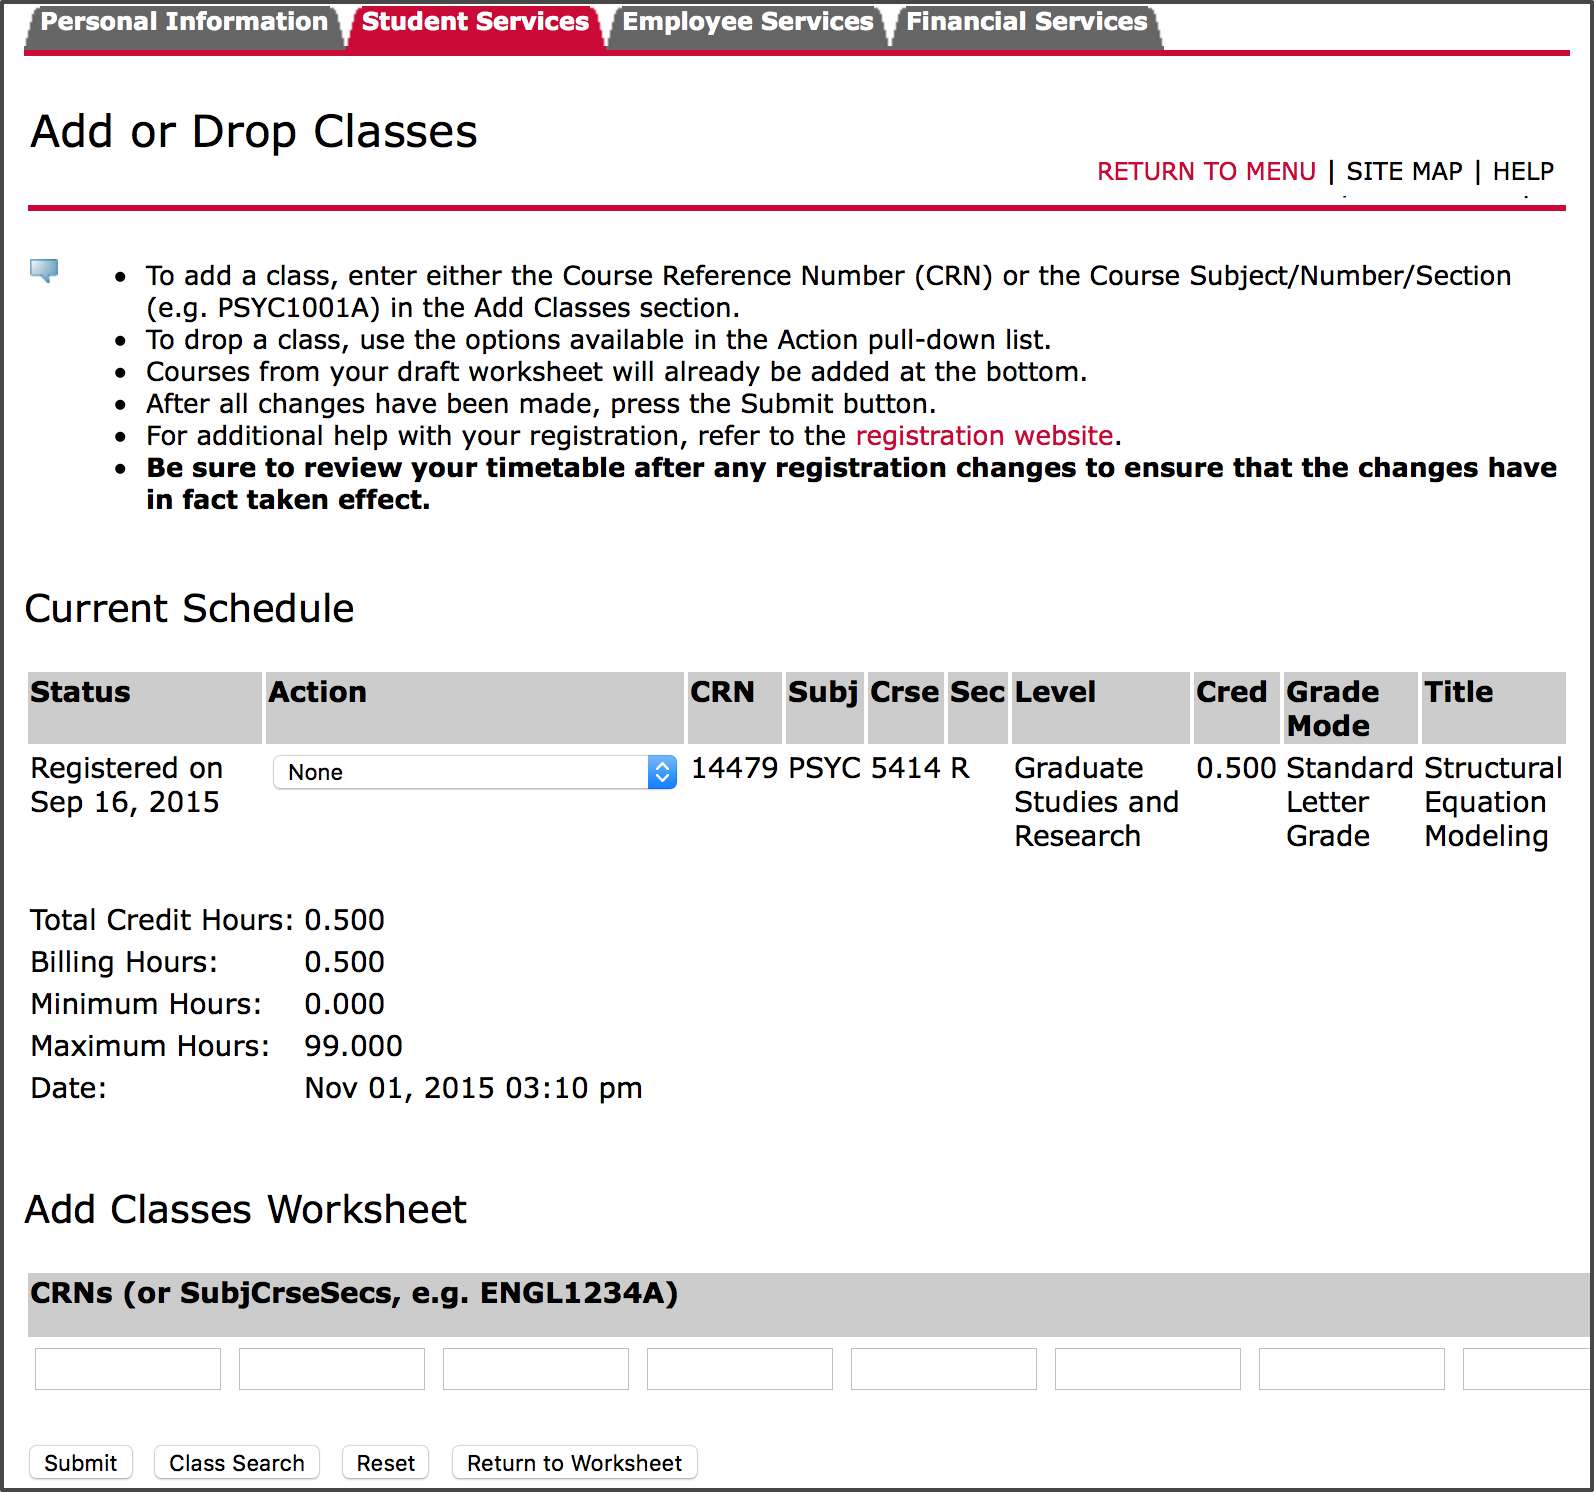
\includegraphics[width=0.8\textwidth]{CarletonScreen.png}
%\end{center}
%\Caption{Add courses view -- Central}
%\end{InlineColumnFigure}
%\vspace{4mm}

\subsubsection*{Critique}
There are a large number of prominent usability flaws in Carleton University's 
Central course-management system. Visibility of common functions on the main 
page is very low, as a long list of hyperlinks contains all the categories (e.g. 
Registration, Student Records etc) requiring the user to read each one until 
they find the correct one. Once a category is selected, then another list of 
hyperlinks to each of the functions in that category is shown (see figure 4). 
Again, the user must read through each one until they find the desired function.


%\begin{InlineColumnFigure}
%\begin{center}
%	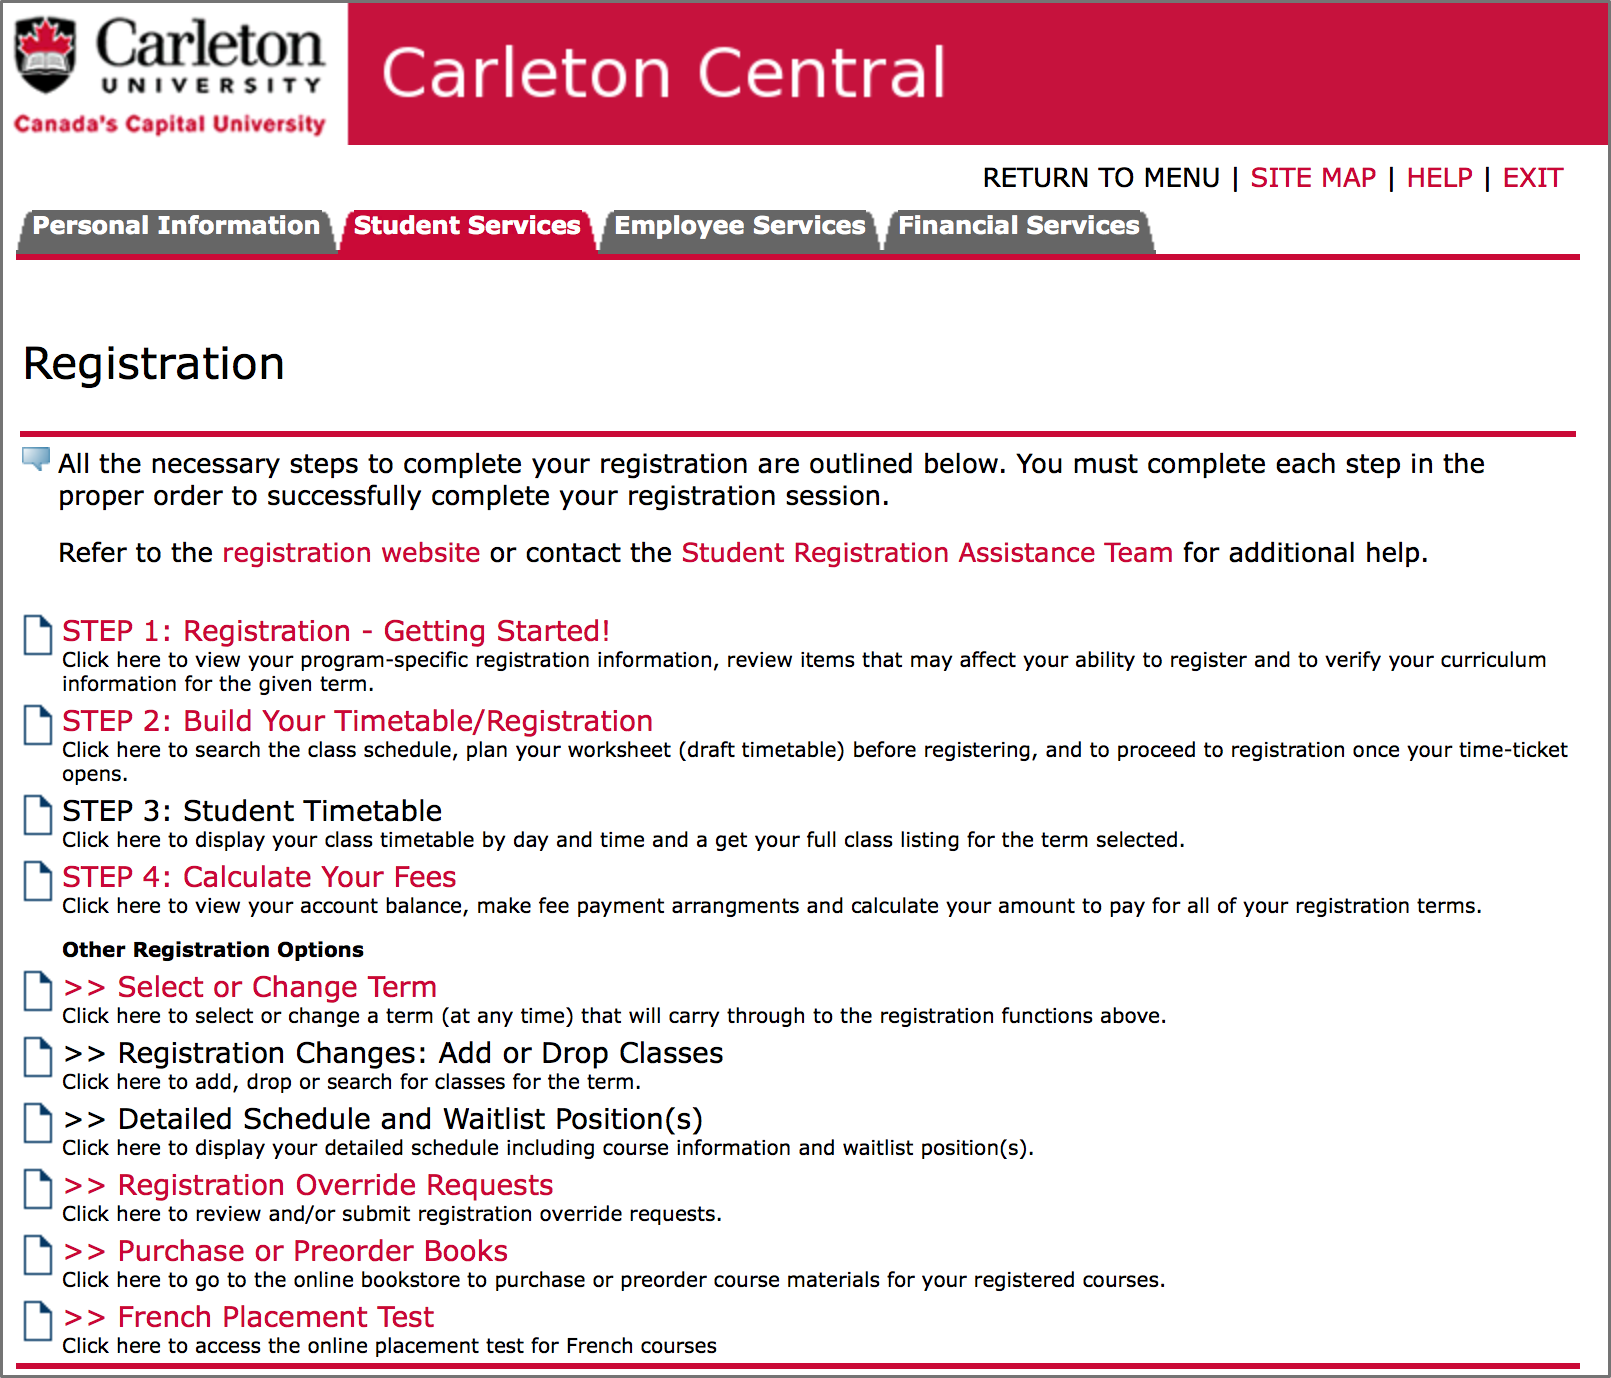
\includegraphics[width=0.9\textwidth]{CarletonScreen2.png}
%\end{center}
%\Caption{Registration main page -- Central}
%\end{InlineColumnFigure}

Another large usability flaw is the poor mapping between many actions. For 
example, when adding a course, the user first enters a course number into one of 
several (unlabeled) input boxes, and then they click the Submit button (see 
figure 3). The submit button is aligned with other buttons for Class Search, 
which takes the user to a separate page, Reset, which undoes their changes, and 
Return to Worksheet which navigates the user to a page showing them their 
preferred courses. These buttons are not all related, and grouping them together 
may confuse the user.

Overall, Central is a relatively unintuitive system, requiring users to spend 
more time finding the information they need through poor mappings and a lack of 
a visual hierarchy.

% =================== SubSection =================== %
\subsection*{Waterloo University -- Quest}
\subsubsection*{Description}
The Quest system is designed to let students manage several aspects 
of their university enrollment, such as course management, financial inquiries, 
and contact information. Students can also sign up for a GO Bus pass, view their 
grades and transcript, and check the status of scholarships and other 
applications. The main page is broken up into 8 collapsible sections, 4 main 
sections (Academics, Finances, Personal Information, Admissions) with another 4 
sections in a sidebar (Holds, Finance Information, Academic Information, Other 
Useful Links). The critique will focus on enrolling in courses and viewing a 
user's course schedule. 

%\begin{InlineColumnFigure}
%\begin{center}
%	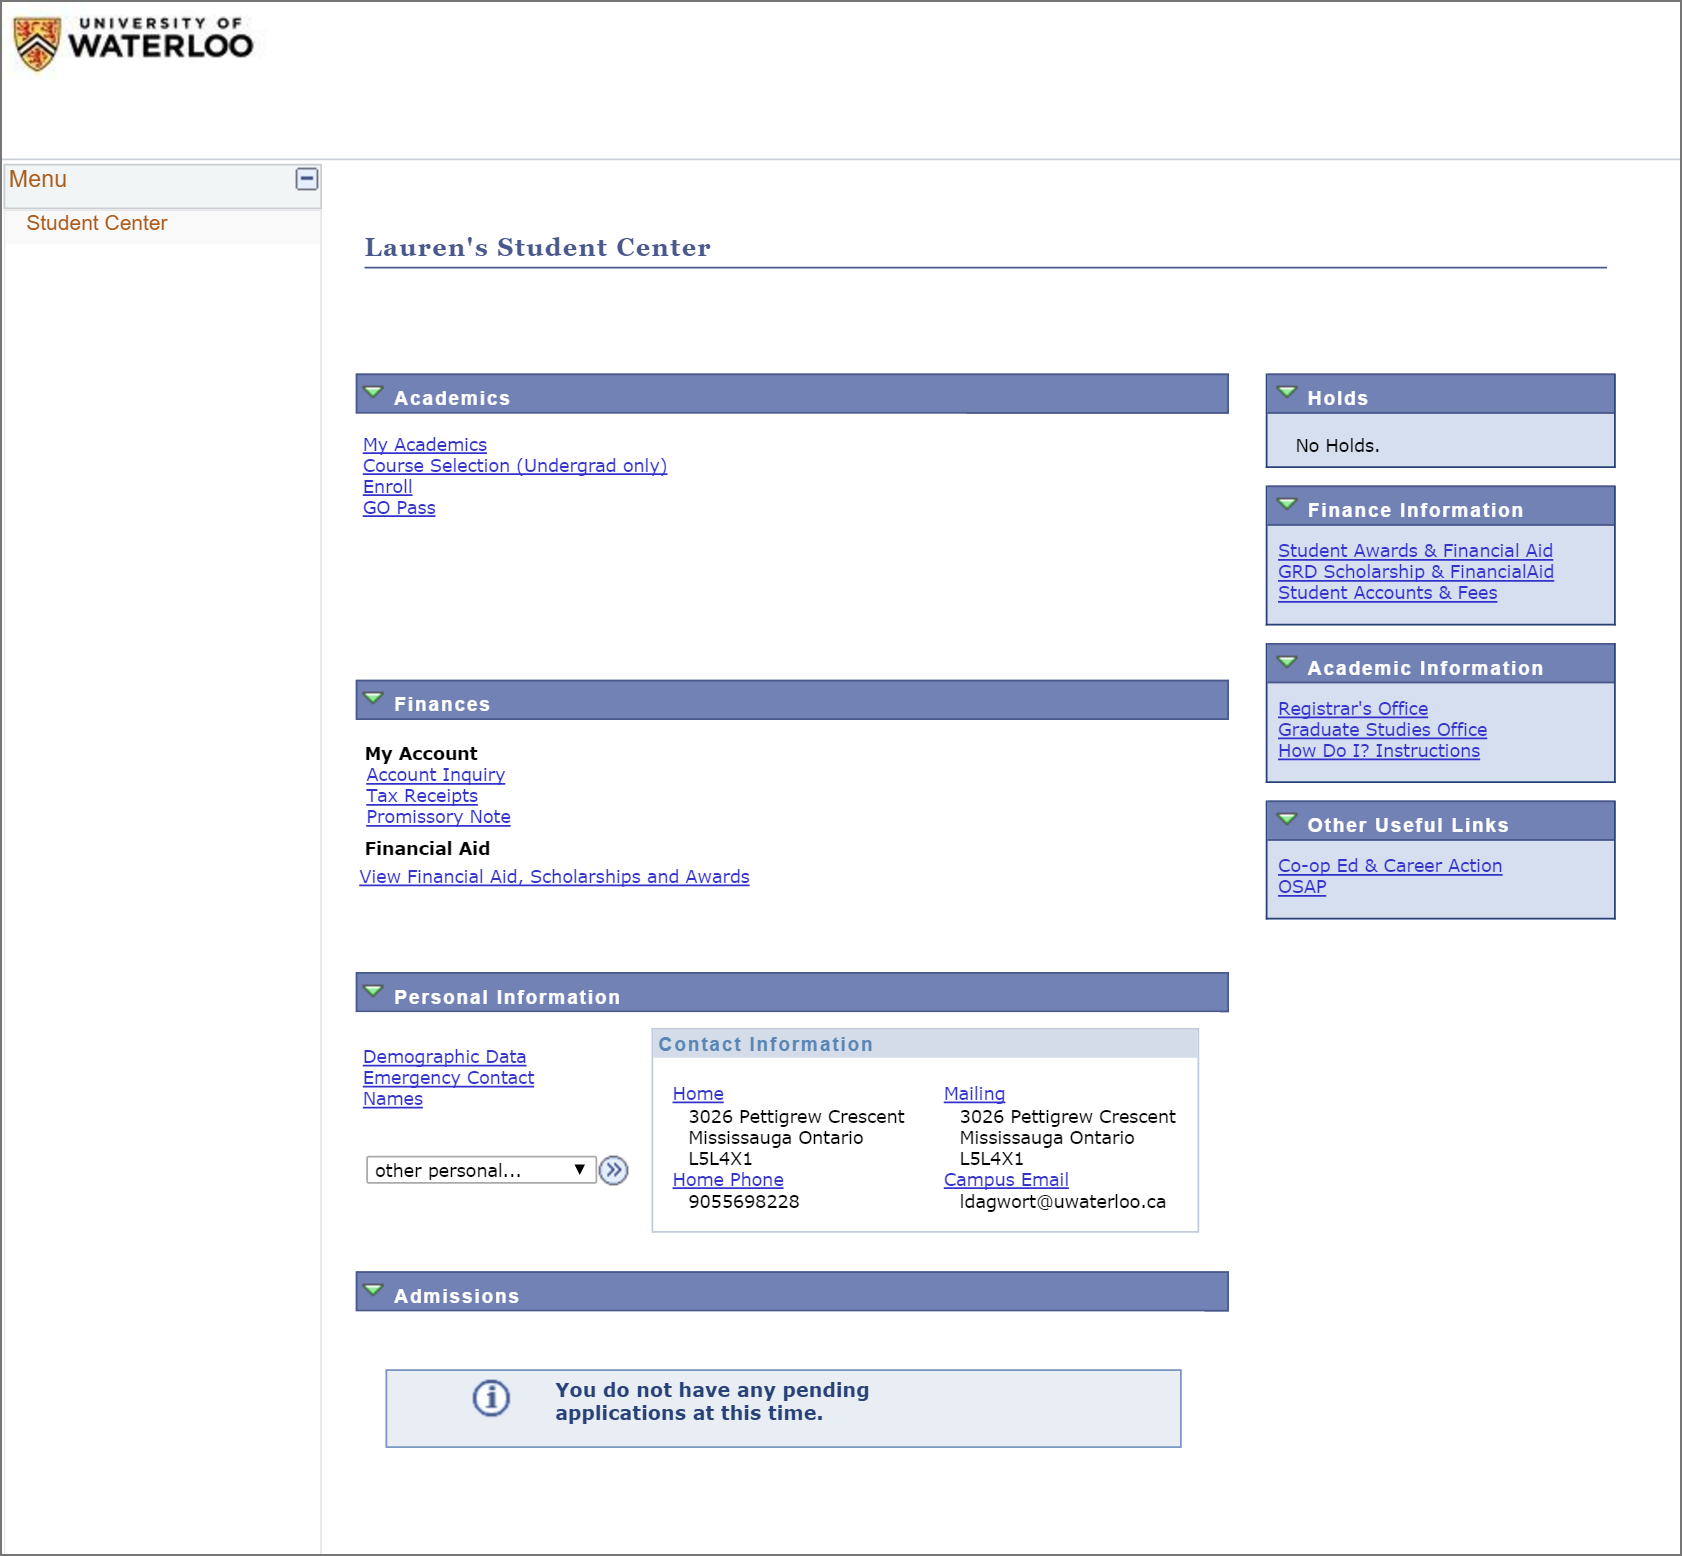
\includegraphics[width=0.9\textwidth]{WaterlooScreen.png}
%\end{center}
%\Caption{Student main page -- Quest}
%\end{InlineColumnFigure}

\subsubsection*{Critique}
Quest has some major usability issues when it comes to providing the user to 
information and functions they can use. The system is notorious for hiding 
options and menus from the user, requiring several screens of drill down menus 
before being able to access any meaningful options. The menus look unfinished or 
poorly formatted, and it is easy to become lost and confused while navigating 
the various pages. Navigation on the main page is done using hyperlinked text, 
while traversing the deeper options is done using blue menu tabs. Native browser 
back and forward commands generally work as expected, which makes navigation a 
little more manageable. 

% =================== Section =================== 
%\section*{Conclusion}
%We have discussed several proposed improvements to a course-management system. 
%These include a dynamic element highlighting the most-needed feature based on 
%several factors, an improved layout with better indicators, and a more 
%intelligent course scheduler. We have also provided a software survey for four 
%Canadian university course-management systems. For each survey we critiqued the 
%software as well as analyzed the two most important features via hierarchical 
%task analyses, presented at the end of this paper.

\end{multicols}
%
%\newpage
%
%\section*{HTA - Mosaic, Enrolling in a Course}
%\begin{center}
%\fbox{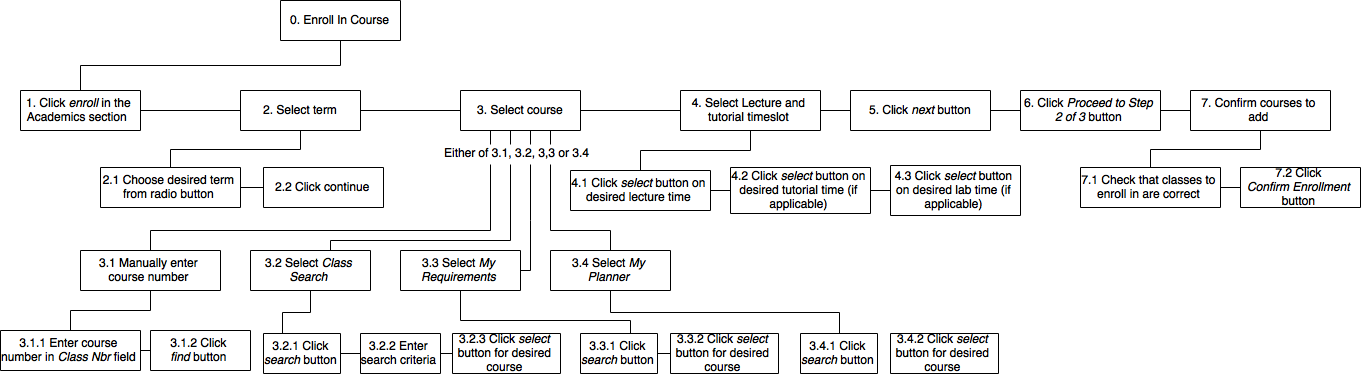
\includegraphics[height=\textheight]{MosaicEnroll.png}}
%\end{center}
%
%\section*{HTA - Mosaic, Viewing Weekly Schedule}
%\begin{center}
%\fbox{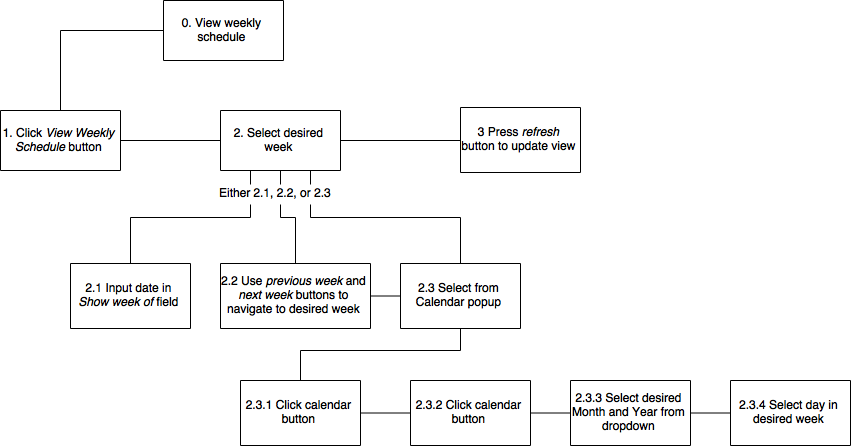
\includegraphics[width=\textwidth]{MosaicViewSchedule.png}}
%\end{center}
%
%\section*{HTA - WebAdvisor, Enrolling in a Course}
%\begin{center}
%\fbox{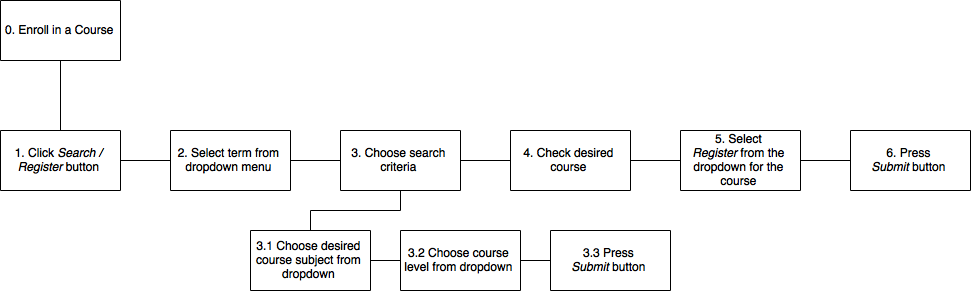
\includegraphics[width=\textwidth]{WebAdvisorEnroll.png}}
%\end{center}
%
%\section*{HTA - WebAdvisor, Viewing Weekly Schedule}
%\begin{center}
%\fbox{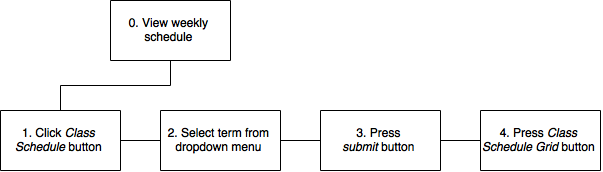
\includegraphics[width=\textwidth]{WebAdvisorViewSchedule.png}}
%\end{center}
%
%\section*{HTA - Central, Enrolling in a Course}
%\begin{center}
%\fbox{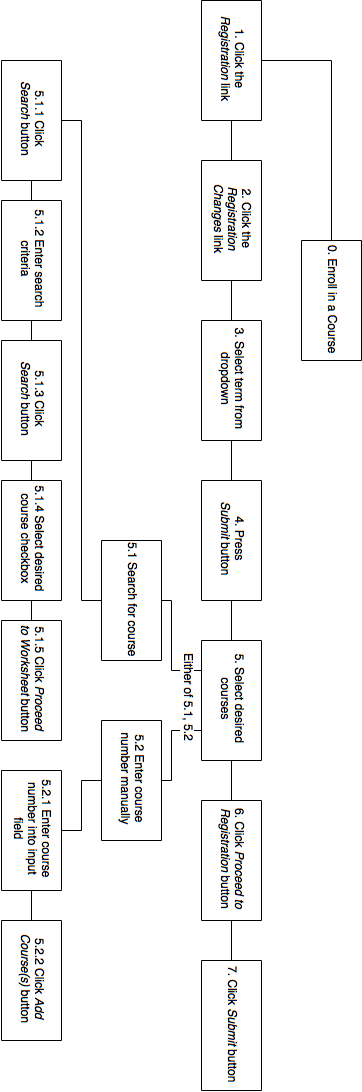
\includegraphics[height=\textheight]{CarletonEnroll.png}}
%\end{center}
%
%\section*{HTA - Central, Viewing Weekly Schedule}
%\begin{center}
%\fbox{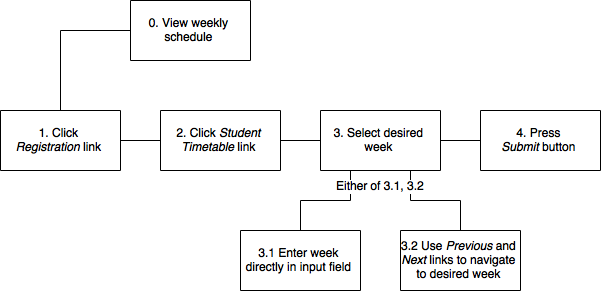
\includegraphics[width=\textwidth]{CarletonViewSchedule.png}}
%\end{center}
%
%\section*{HTA - Quest, Enrolling in a Course}
%\begin{center}
%\fbox{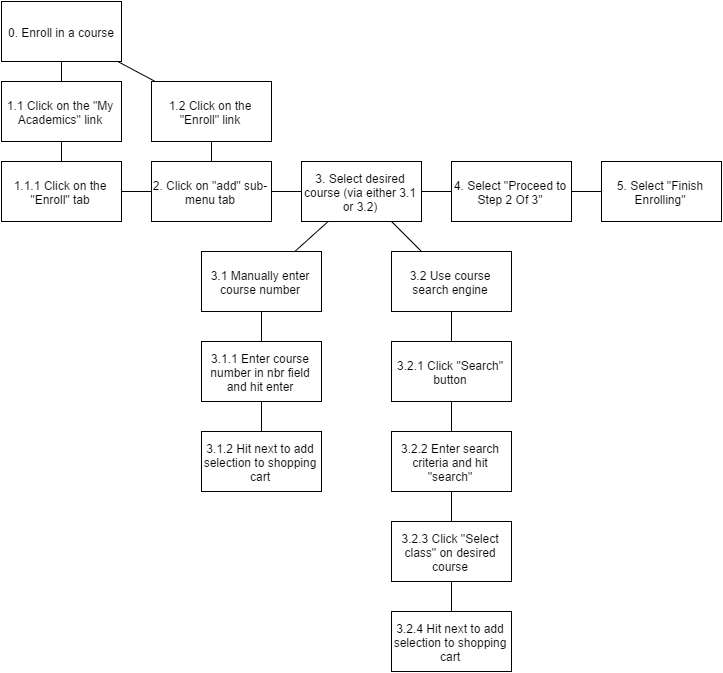
\includegraphics[width=\textwidth]{WaterlooEnroll.png}}
%\end{center}
%
%\section*{HTA - Quest, Viewing Weekly Schedule}
%\begin{center}
%\fbox{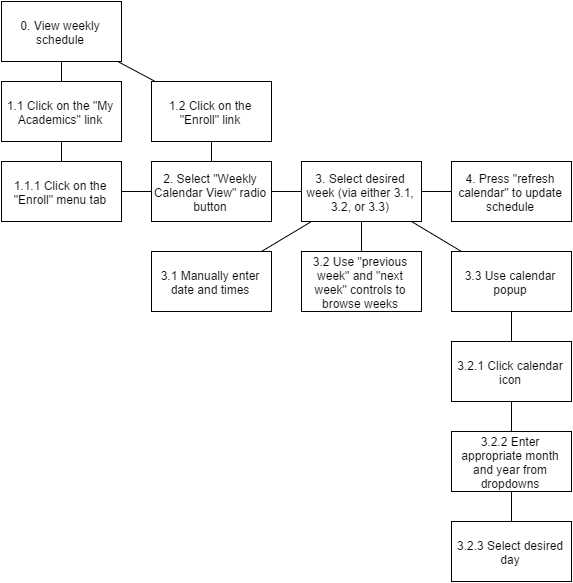
\includegraphics[width=\textwidth]{WaterlooSchedule.png}}
%\end{center}


\section*{Personas}\vspace{2mm}
%. The \textbf{design project} involves creating a new user interface and user experience for university student management software. The focus has been on developing an improved system design as compared to McMaster University's current Mosaic software. Other university's systems have been researched and studied in previous milestones, and those results have informed design decisions for our replacement.\\

This document initially presents the personas used to develop our design.These personas are based off of the \emph{Persona Template} as linked from the assignment outline from McMaster University, COMP SCI 4HC3 These personas were created to archetype the most common user types, and have been integral to developing a product that will satisfy all of them.\\

%Following the personas, we've included two HTA's to highlight the two most important functions of the software -- enrolling in courses and viewing one's class schedule. The simplicity of the HTA's as compared to those created from existing systems is an attestation to our efforts to reduce the complexity of core interactions with the product.\\
%
%Finally, design documents for each page of the system are included. These include several revisions for each page (some underwent more revisions than others). Along with each revision we've included a brief description of what motivated our changes, and how they improve upon the design. Initial revisions for each page were sketched on paper for rapid prototyping, and subsequent revisions were created in Photoshop.

%\vspace{5mm}
%%============================= Persona 1 ======================================%
%\hrule
%\vspace{4mm}
%\subsection{Persona 1 -- Primary persona}
%\vspace{11mm}

\subsection*{Trevor Clark}
%\vspace{4mm}

\begin{minipage}{60mm}

\includegraphics[width=60mm]{Trevor.jpg}
\begin{center}
\emph{``When do classes start?"}
\end{center}
\end{minipage}
\begin{minipage}{\textwidth}
\begin{itemize}
\item Born: London, ON
\item Age: 22
\item 3rd Year Engineering Student at McMaster
\end{itemize}
\end{minipage}\\

Trevor is a third year Civil Engineering student at McMaster. He currently lives 10 minutes away from campus with some friends he met in first year. Trevor's parents are paying for his tuition and he has a student loan which he uses to pay for rent and food.

Trevor is unorganized and rarely goes to class. He also forgets to hand in assignments on time. Trevor is not a part of any clubs and prefers to spend his free time with his housemates playing video games.

Trevor has trouble remembering important dates, like his course selection or when his exams are. When he searches for information, he usually gives up after five minutes if he cannot find what he is looking for. Trevor would like it if the new course management system was quick and easy to use. He also would not mind it if certain information was made more accessible during certain times of the year (easy to see link to exam schedule around exam season).

%%============================= Persona 2 ======================================%
%\hrule
%\vspace{2mm}
%\subsection{Persona 2 -- Secondary persona}
%\vspace{11mm}

\subsection*{Candice Smith}
%\vspace{4mm}

\begin{minipage}{80mm}

\includegraphics[width=80mm]{Candice.jpg}
\begin{center}
\emph{``I don't know what electives I want to take for university next year"}
\end{center}
\end{minipage} \hfill
\begin{minipage}{\textwidth}
\begin{itemize}
\item Born: Oakville, ON
\item Age: 18
\item Grade 12 High School Student
\end{itemize}
\end{minipage}\\


Candice has been accepted to the chemistry program at McMaster. Candice currently lives at home with her parents and will be moving into residence in the fall. Her parents are paying for her tuition, but Candice is paying for her residence and meal plan. Candice works part time at the Fortinos in her home town to save up money so she can go to the movies whenever new movies come out.

Candice has done well in all of her classes in high school and is a part of several high school groups; such as the volleyball team, track and field team and the Harry Potter fan club.

Candice has several electives that she can take, but she cannot decide which ones to enrol in. She has heard that she can change courses during the first couple weeks of class and plans on doing that if she ends up changing her mind. Candice has already made a list of classes she would like to take in her first year and is waiting for the course registration to open up. Candice would like the new course management system to allow her to browse all the courses available to her and would like it if there were descriptions for each course that she could read before she registers.

%%============================= Persona 3 ======================================%
%\hrule
%\vspace{2mm}
%\subsection{Persona 3 -- Secondary persona}
%\vspace{11mm}

\subsection*{Adrian Lopez}
%\vspace{4mm}

\begin{minipage}{70mm}

\includegraphics[width=70mm]{Adrian.png}
\begin{center}
\emph{``I have a lot of new things to get used to in Canada"}
\end{center}
\end{minipage}\hfill
\begin{minipage}{\textwidth}
\begin{itemize}
\item Born: Mexico City, Mexico
\item Age: 20
\item 2nd Year Geography Student on Exchange to McMaster
\end{itemize}
\end{minipage}\\

Adrian is a geography student from Mexico on exchange at McMaster for the year. Adrian is living in a house 20 minutes away from campus with other students in the foreign exchange program. Adrian's tuition is being paid for by a grant he received for being a part of the foreign exchange program. His parents are giving him some money for rent and food but Adrian has to pay for some of it himself. Adrian is a hard working individual during the week and can be found in the Thode library between classes. Adrian likes to get all of his assignments done during the week so he can spend his weekend going to clubs with his housemates and friends.

Adrian is a part of the improv club which he regularly goes to. Adrian has chosen a light course load this year as he would like some time to experience Canada before he goes back to Mexico next September.

Since English is not Adrian's first language he sometimes has trouble reading and understanding websites that are primarily text, and he can get confused while navigating to the information he is looking for. Adrian would like it if the new course management system was easy to navigate and intuitive enough that he doesn't need to read an instruction manual to know how to use it.

\newpage
\begin{multicols}{2}
\section*{Usability Tests}
\subsection*{Results}
\subsection*{Discussion}
\subsection*{Conclusion}
\end{multicols}

\end{document}
